\documentclass[12pt, a4paper]{article}
\usepackage[finnish]{babel}
\usepackage[utf8x]{inputenc}
\usepackage[T1]{fontenc}
\usepackage{lmodern}
\usepackage[pdftex]{graphicx}
\usepackage[]{epsfig}
\usepackage[verbose]{layout}
\usepackage{verbatim}
\usepackage{float}
\author{Katja Matilainen}
\title{Taivaanmekaniikan kotitehtävät}
\date{Vuodelta: En edes muista}

\begin{document}
\begin{titlepage}
\maketitle
\end{titlepage}

\section[Tehtävä 1]{Marsin rata taivaalla vuosina 2000-2020}
Ensimmäisessä tehtävässä selvitettiin Tähtitieteen perusteet -kirjasta löytyvän D.12 -taulukon rataelementtien avulla Marsin rata Maan taivaalla vuosien 2000-2020 aikana.

Tehtävä ratkaistiin IDL:llä tehdyllä 'mars.pro' -ohjelmalla, jonka sisältö on esitetty kappaleessa \ref{Koodi1}. Ohjelmassa käytettiin hyväksi valmista 'elem\_to\_rv.pro' -aliohjelmaa, joka laskee annetuista rataelementeistä heliosentrisen paikkavektorin.

\subsection[Ekliptikarata]{Marsin rata Maan ratatasokoordinaatistossa}\label{Ekliptika}
Kuvassa \ref{Kuva1} on esitetty ohjelmasta 'mars.pro' lopputuloksena saatu Marsin rata Maan ratatasokoordinaatistossa.

\begin{figure}[H]
\centerline{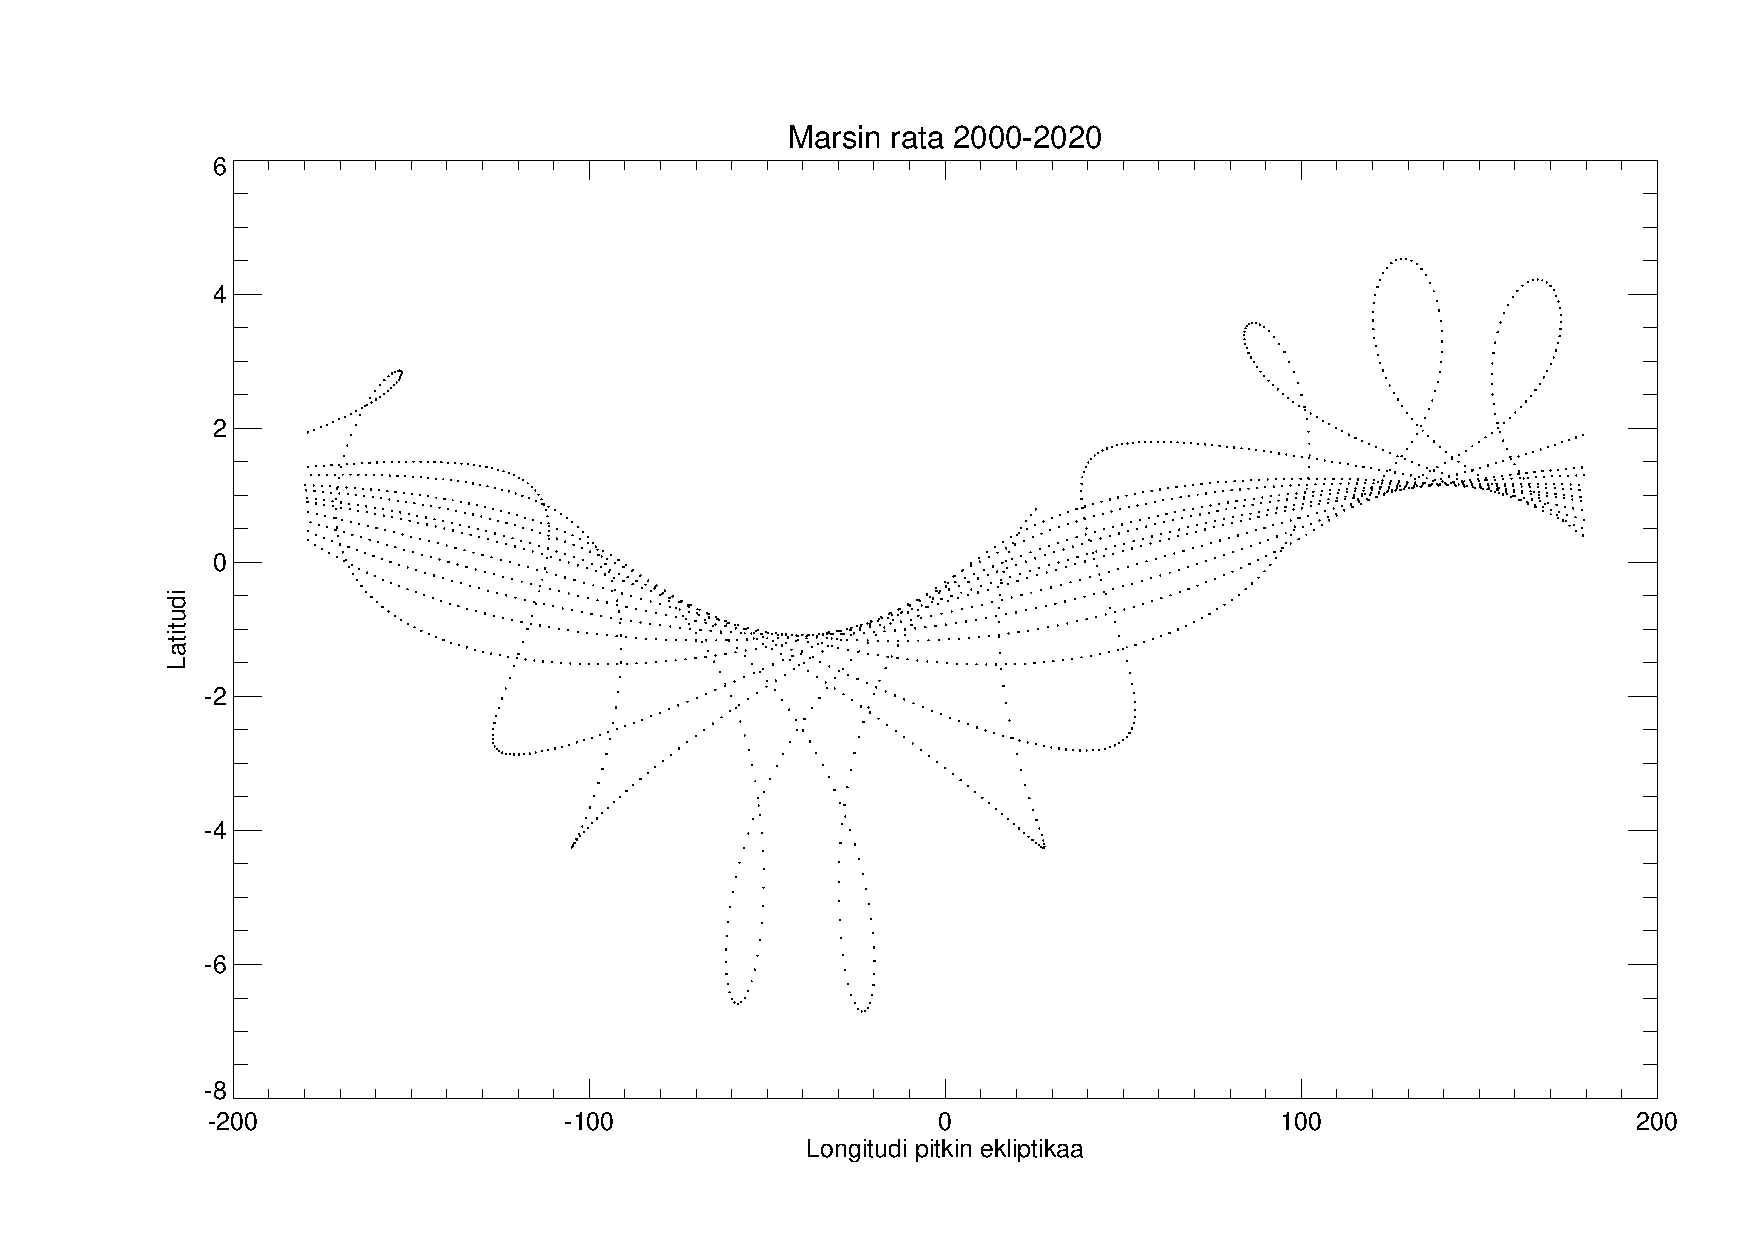
\includegraphics[page=1,angle=0,width=0.8\paperwidth]{mars.pdf}}
\caption{Marsin rata Maan ratatasokoordinaatistossa vuosina 2000-2020}
\label{Kuva1}
\end{figure}

\newpage
\subsection[Ekvaattorirata]{Marsin rata Maan ekvatoriaalisessa koordinaatistossa}\label{Ekvaattori}
Maan ekvaattorijärjestelmässä Marsin paikkaa ei voida yhtä yksikäsitteisen selkeästi esittää yhden kuvaajan avulla. Sen sijaan kuvissa \ref{Kuva2} ja \ref{Kuva3} on esitetty erikseen ohjelmassa 'mars.pro' lasketut Marsin deklinaatio ja rektaskensio ajan funktiona.

Saatuja laskennallisia arvoja (katkoviiva) verrattiin astro -kirjastosta saatuihin tarkkoihin arvoihin (neliösymbolit).

\begin{figure}[H]
\centerline{\includegraphics[page=2,angle=0,width=0.8\paperwidth]{mars.pdf}}
\caption{Marsin deklinaatio}
\label{Kuva2}
\end{figure}

\begin{figure}[H]
\vspace*{-3cm}\centerline{\includegraphics[page=3,angle=0,width=0.8\paperwidth]{mars.pdf}}
\caption{Marsin rektaskensio}
\label{Kuva3}
\end{figure}
\vspace*{1cm}

Lopuksi deklinaation ja rektaskension arvoja verrattiin JPL-ephemerideihin, ja esittettiin niiden virheet ajan funktiona (kuva \ref{Kuva4}).

\newpage
\begin{figure}[H]
\vspace*{-3.5cm}\centerline{\includegraphics[page=4,angle=0,width=0.8\paperwidth]{mars.pdf}}
%\caption{Deklinaation virhe}
%\label{Kuva4}
\end{figure}

\begin{figure}[H]
\vspace*{-2.5cm}\centerline{\includegraphics[page=5,angle=0,width=0.8\paperwidth]{mars.pdf}}
\caption{Deklinaation ja rektaskension virhe}
\label{Kuva4}
\end{figure}

\newpage
\section[Tehtävä 2]{Numeerinen integrointi}
Toisessa tehtävässä oli tarkoitus laskea kappaleen rata erilaisilla numeerisilla menetelmillä $1/r^2$ ja $1/r^3$ -muotoisissa voimakentissä, ja verrata saatuja tuloksia analyyttiseen rataan. Samalla seurattiin energian ja impulssimomentin säilymistä eri menetelmillä.

Tehtävässä käytettiin valmiita aliohjelmia 'kepler.pro' sekä 'inte\_simple\_f.pro', joista jälkimmäistä muokattiin ratkaisemaan tarvittaessa myös kappaleen analyyttinen rata. Myös muutamia muita muutoksia tehtiin ohjelmaan.

\subsection[Tehtävä 2a]{Kahden kappaleen liike $1/r^2$ -voimakentässä}
Kappaleen rata laskettiin neljällä eri menetelmällä eri eksentrisyyden arvoille ($e=0$, $e=0.5$ ja $e=0.9$) niin, että isoakselin puolikkaan suurudeksi valittiin $a=1$ ja systeemin massa skaalattiin arvoon $\mu=1$.

Laskelmat toistettiin aika-askeleen arvoilla $dt=0.01P$, $dt=0.001P$ ja $dt=0.0001P$ niin, että integroinnin kokonaisaika oli $t=10P$.

Jo pelkkien ratojen perusteella voidaan päätellä suuntaa-antavasti jotain integrointimenetelmien tarkkuudesta. Kuvista 5-18 nähdään, että ensimmäisen asteen Taylorin menetelmä on kaukana analyyttisesta ratkaisusta, ja ei tuota suljettua rataa suurilla aika-askeleen $dt$ ja eksentrisyyden $e$ arvoilla.

Toisen asteen Taylorin menetelmä on huomattavasti ensimmäisen asteen menetelmää luotettavampi, mutta molemmat häviävät kirkkaasti Runge-Kuttalle, jonka antama tulos on hyvin lähellä analyyttista rataa kaikilla käytetyillä aika-askeleen arvoilla. Vain käyttämällä yhtä aikaa suurta eksentrisyyden ($e \geq 0.9$) ja aika askeleen ($dt \geq 0.01P$) arvoa myös Runge-Kuttan menetelmä on epäluotettava.

Saman tuloksen näkee myös energian ja impulssimomentin säilymisestä.

\newpage
\subsubsection{Kappaleen rata, kun $e=0$ ja $dt=0.01P$}
%\newpage
\begin{figure}[H]
\vspace*{-1.5cm}
\includegraphics[page=1,angle=0,width=0.7\paperwidth]{numorb.pdf}%}
\end{figure}

\begin{figure}[H]
\vspace*{-2.5cm}
\includegraphics[page=2,angle=0,width=0.7\paperwidth]{numorb.pdf}%}
\caption{Analyyttinen rata ja 1. kertaluvun Taylorin menetelmä, $dt=0.01P$}
\end{figure}

\newpage
\begin{figure}[H]
%\vspace*{-2.5cm}
\includegraphics[page=3,angle=0,width=0.7\paperwidth]{numorb.pdf}%}
\end{figure}

\begin{figure}[H]%\centerline{
\vspace*{-2.5cm}
\includegraphics[page=4,angle=0,width=0.7\paperwidth]{numorb.pdf}%}
\caption{2. kertaluvun Taylorin menetelmä ja Runge-Kutta, $dt=0.01P$}
\end{figure}

\newpage
\subsubsection{Energian säilyminen, kun $e=0$ ja $dt=0.01$}
\begin{figure}[H]
\vspace*{-1cm}
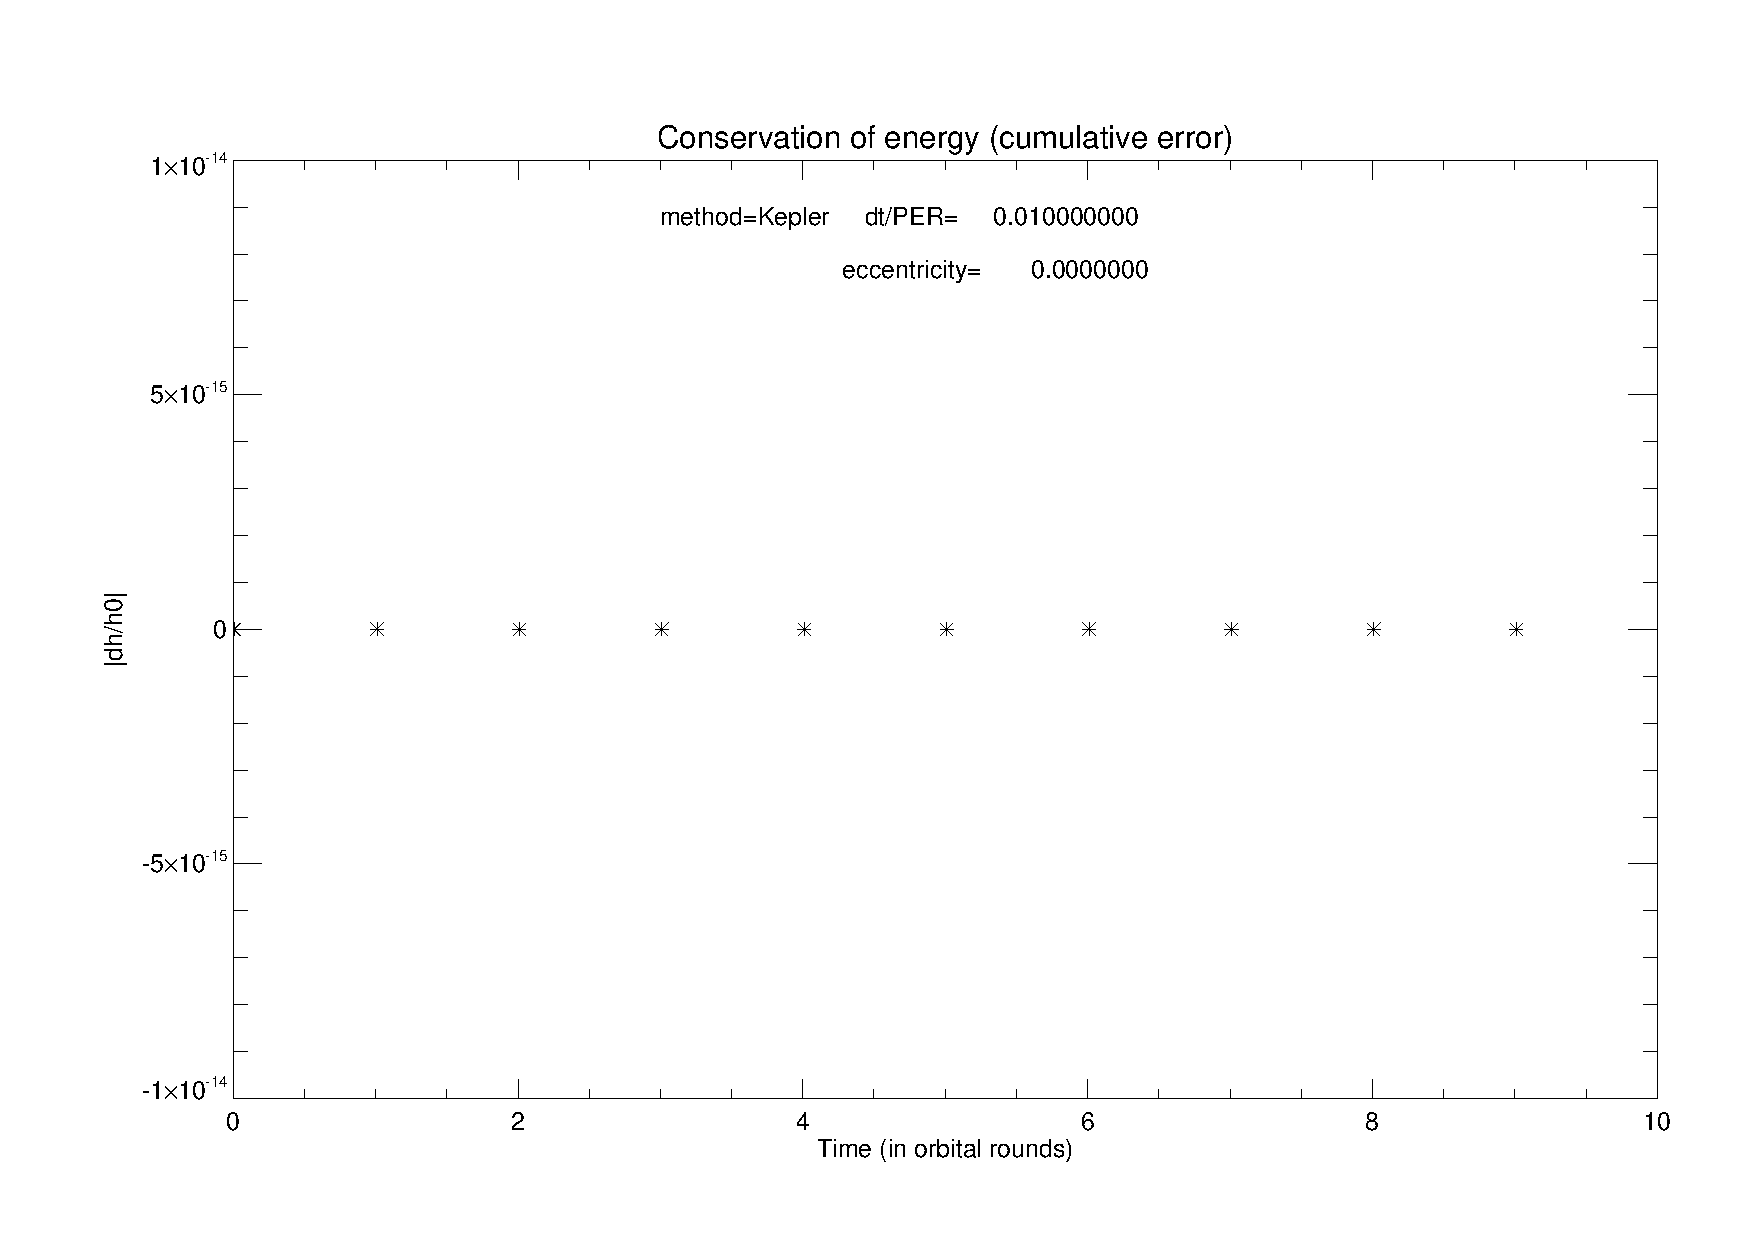
\includegraphics[page=1,angle=0,width=0.7\paperwidth]{numorb_energy_e0dt01.pdf}
\end{figure}

\begin{figure}[H]%\centerline{
\vspace*{-2cm}
\includegraphics[page=2,angle=0,width=0.7\paperwidth]{numorb_energy_e0dt01.pdf}%}
\caption{Analyyttinen rata ja 1. kertaluvun Taylorin menetelmä $dt=0.01P$}
\end{figure}

\newpage
\begin{figure}[H]%\centerline{
%\vspace*{-2.5cm}
\includegraphics[page=3,angle=0,width=0.7\paperwidth]{numorb_energy_e0dt01.pdf}%}
\end{figure}

\begin{figure}[H]%\centerline{
\vspace*{-2cm}
\includegraphics[page=4,angle=0,width=0.7\paperwidth]{numorb_energy_e0dt01.pdf}%}
\caption{2. kertaluvun Taylorin menetelmä ja Runge-Kutta, $dt=0.01P$}
\end{figure}

\newpage
\subsubsection{Kappaleen rata, kun $e=0.5$ ja $dt=0.01P$}
%\newpage
\begin{figure}[H]%\centerline{
\vspace*{-1.5cm}
\includegraphics[page=5,angle=0,width=0.7\paperwidth]{numorb.pdf}%}
%\caption{Kepler-liike, analyyttinen rata}
\end{figure}\label{ke05}

\begin{figure}[H]%\centerline{
\vspace*{-2.5cm}
\includegraphics[page=6,angle=0,width=0.7\paperwidth]{numorb.pdf}%}
\caption{Analyyttinen rata ja 1. kertaluvun Taylorin menetelmä, $dt=0.01P$}
\end{figure}\label{t1e05}

%\newpage
\begin{figure}[H]%\centerline{
\vspace*{-1.5cm}
\includegraphics[page=7,angle=0,width=0.7\paperwidth]{numorb.pdf}%}
\end{figure}\label{t2e05}

\begin{figure}[H]%\centerline{
\vspace*{-2.5cm}
\includegraphics[page=8,angle=0,width=0.7\paperwidth]{numorb.pdf}%}
\caption{2. kertaluvun Taylorin menetelmä ja Runge-Kutta, $dt=0.01P$}
\end{figure}\label{rk4e05}

\newpage
\subsubsection{Energian säilyminen, kun $e=0.5$ ja $dt=0.01$}
\begin{figure}[H]
\vspace*{-1cm}
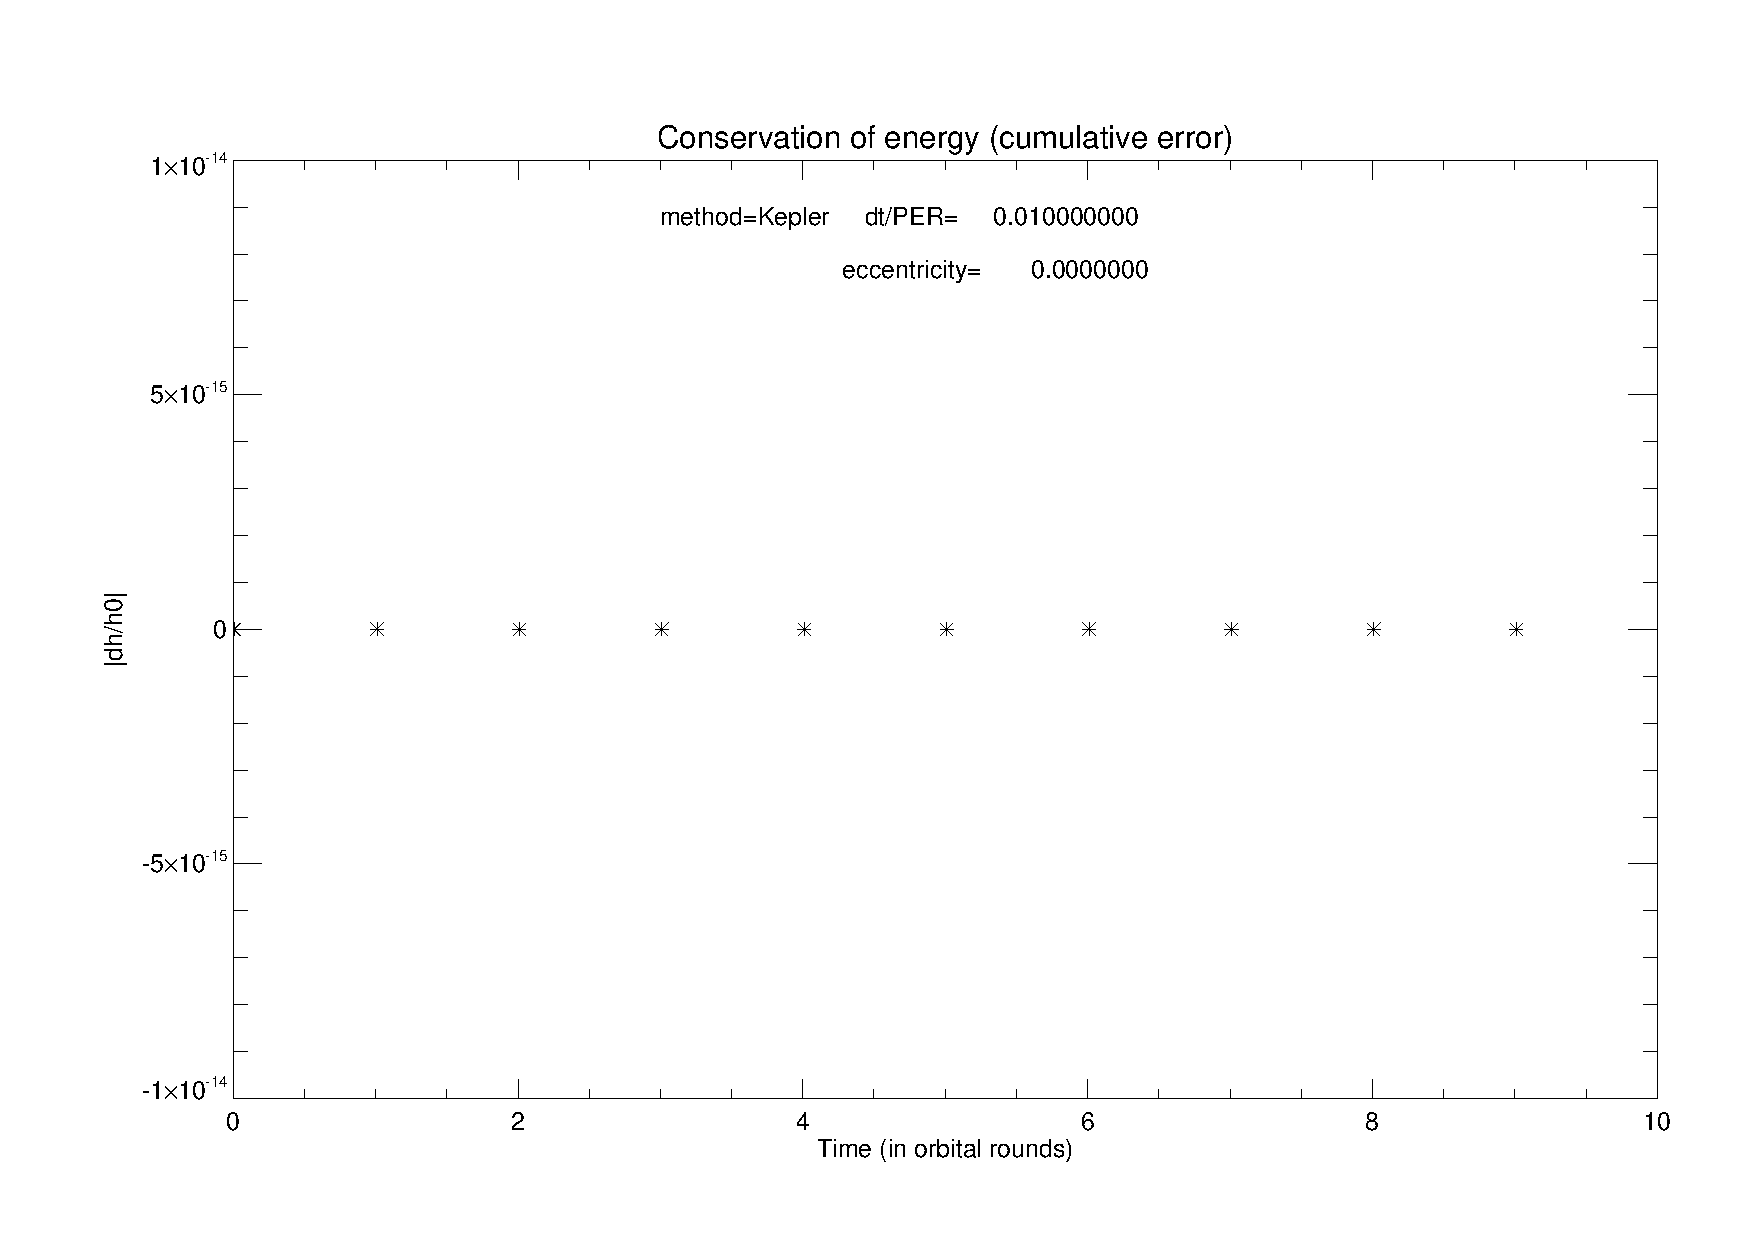
\includegraphics[page=1,angle=0,width=0.7\paperwidth]{numorb_energy_e0dt01.pdf}
\end{figure}

\begin{figure}[H]%\centerline{
\vspace*{-2cm}
\includegraphics[page=2,angle=0,width=0.7\paperwidth]{numorb_energy_e5dt01.pdf}%}
\caption{Analyyttinen rata ja 1. kertaluvun Taylorin menetelmä $dt=0.01P$}
\end{figure}

\newpage
\begin{figure}[H]%\centerline{
%\vspace*{-2.5cm}
\includegraphics[page=3,angle=0,width=0.7\paperwidth]{numorb_energy_e5dt01.pdf}%}
\end{figure}

\begin{figure}[H]%\centerline{
\vspace*{-2cm}
\includegraphics[page=4,angle=0,width=0.7\paperwidth]{numorb_energy_e5dt01.pdf}%}
\caption{2. kertaluvun Taylorin menetelmä ja Runge-Kutta, $dt=0.01P$}
\end{figure}

\newpage
\subsubsection{Kappaleen rata, kun $e=0.9$ ja $dt=0.01P$}
%\newpage
\begin{figure}[H]%\centerline{
\vspace*{-1.5cm}
\includegraphics[page=9,angle=0,width=0.7\paperwidth]{numorb.pdf}%}
%\caption{Kepler-liike, analyyttinen rata}
\end{figure}\label{ke09}

\begin{figure}[H]%\centerline{
\vspace*{-2.5cm}
\includegraphics[page=10,angle=0,width=0.7\paperwidth]{numorb.pdf}%}
\caption{Analyyttinen rata ja 1. kertaluvun Taylorin menetelmä, $dt=0.01P$}
\end{figure}\label{t1e09}

\newpage
\begin{figure}[H]%\centerline{
%\vspace*{-2.5cm}
\includegraphics[page=11,angle=0,width=0.7\paperwidth]{numorb.pdf}%}
\end{figure}\label{t2e09}

\begin{figure}[H]%\centerline{
\vspace*{-2.5cm}
\includegraphics[page=12,angle=0,width=0.7\paperwidth]{numorb.pdf}%}
\caption{2. kertaluvun Taylorin menetelmä ja Runge-Kutta, $dt=0.01P$}
\end{figure}\label{rk4e09}

\newpage
\subsubsection{Energian säilyminen, kun $e=0.9$ ja $dt=0.01$}
\begin{figure}[H]
\vspace*{-1cm}
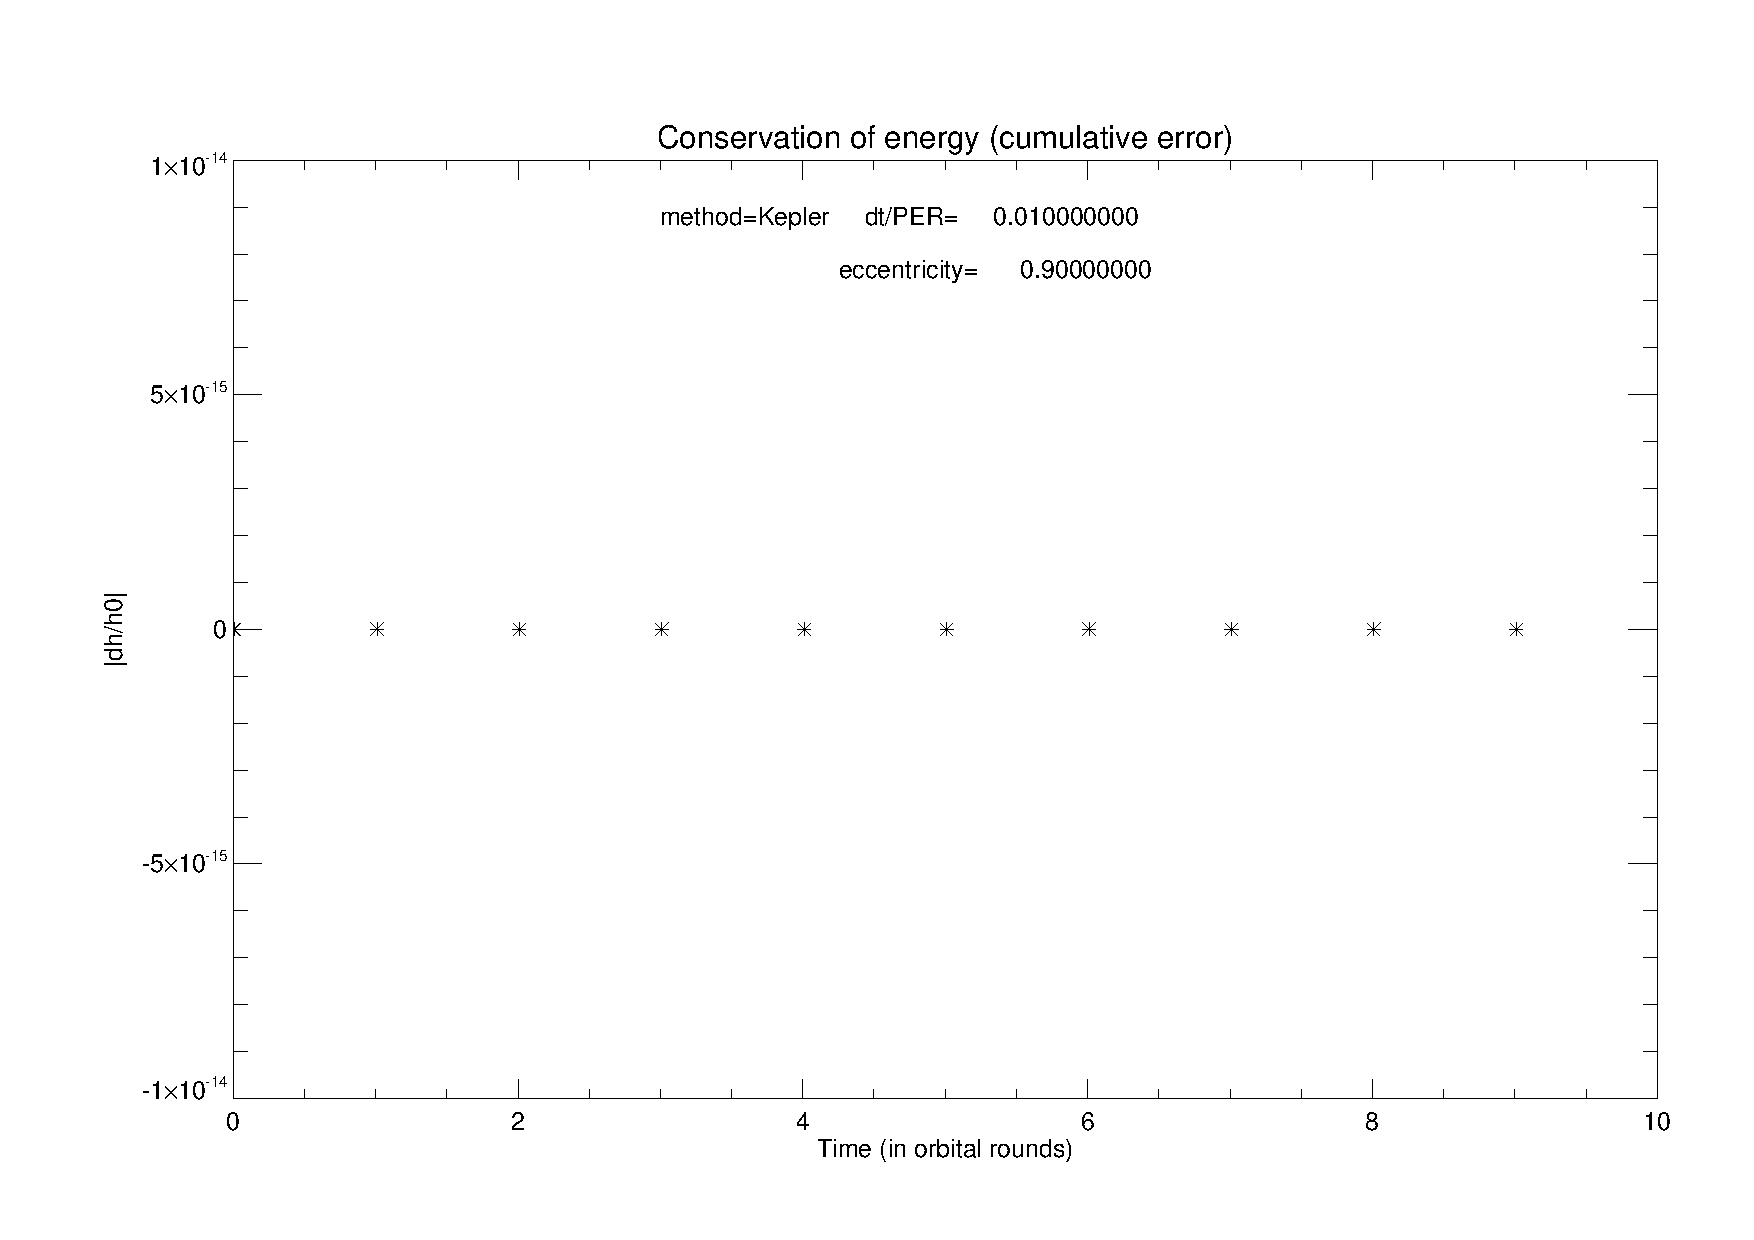
\includegraphics[page=1,angle=0,width=0.7\paperwidth]{numorb_energy_e9dt01.pdf}
\end{figure}

\begin{figure}[H]%\centerline{
\vspace*{-2cm}
\includegraphics[page=2,angle=0,width=0.7\paperwidth]{numorb_energy_e9dt01.pdf}%}
\caption{Analyyttinen rata ja 1. kertaluvun Taylorin menetelmä $dt=0.01P$}
\end{figure}

\newpage
\begin{figure}[H]%\centerline{
%\vspace*{-2.5cm}
\includegraphics[page=3,angle=0,width=0.7\paperwidth]{numorb_energy_e9dt01.pdf}%}
\end{figure}

\begin{figure}[H]%\centerline{
\vspace*{-2cm}
\includegraphics[page=4,angle=0,width=0.7\paperwidth]{numorb_energy_e9dt01.pdf}%}
\caption{2. kertaluvun Taylorin menetelmä ja Runge-Kutta, $dt=0.01P$}
\end{figure}

\newpage
\subsubsection{Kappaleen rata, kun $e=0$ ja $dt=0.001P$}
\begin{figure}[H]
\vspace*{-1.5cm}
\includegraphics[page=13,angle=0,width=0.7\paperwidth]{numorb.pdf}
\end{figure}

\begin{figure}[H]%\centerline{
\vspace*{-2.5cm}
\includegraphics[page=14,angle=0,width=0.7\paperwidth]{numorb.pdf}%}
\caption{Analyyttinen rata ja 1. kertaluvun Taylorin menetelmä, $dt=0.001P$}
\end{figure}

\newpage
\begin{figure}[H]%\centerline{
%\vspace*{-2.5cm}
\includegraphics[page=15,angle=0,width=0.7\paperwidth]{numorb.pdf}%}
\end{figure}

\begin{figure}[H]%\centerline{
\vspace*{-2.5cm}
\includegraphics[page=16,angle=0,width=0.7\paperwidth]{numorb.pdf}%}
\caption{2. kertaluvun Taylorin menetelmä ja Runge-Kutta, $dt=0.001P$}
\end{figure}

\newpage
\subsubsection{Energian säilyminen, kun $e=0.0$ ja $dt=0.001$}
\begin{figure}[H]
\vspace*{-1cm}
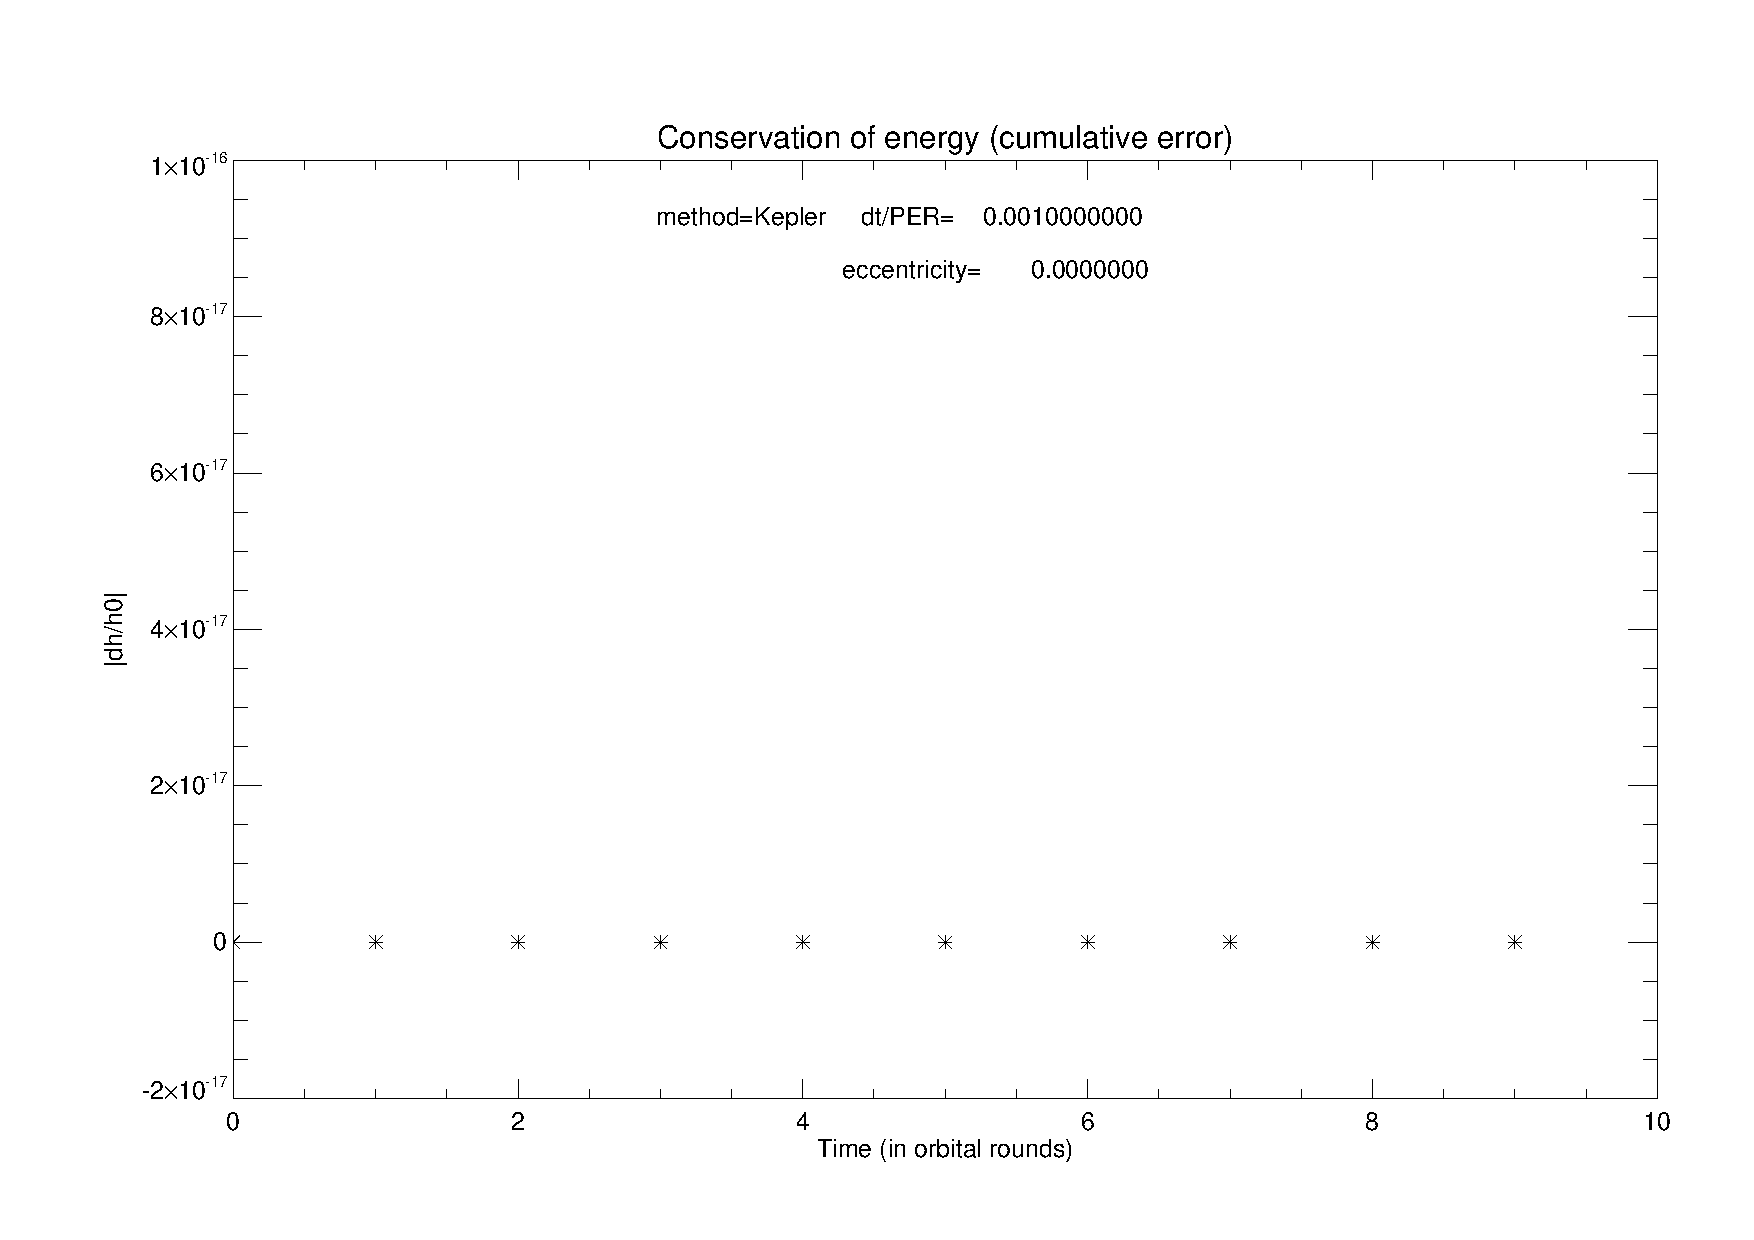
\includegraphics[page=1,angle=0,width=0.7\paperwidth]{numorb_energy_e0dt001.pdf}
\end{figure}

\begin{figure}[H]%\centerline{
\vspace*{-2cm}
\includegraphics[page=2,angle=0,width=0.7\paperwidth]{numorb_energy_e0dt001.pdf}%}
\caption{Analyyttinen rata ja 1. kertaluvun Taylorin menetelmä $dt=0.01P$}
\end{figure}

\newpage
\begin{figure}[H]%\centerline{
%\vspace*{-2.5cm}
\includegraphics[page=3,angle=0,width=0.7\paperwidth]{numorb_energy_e0dt001.pdf}%}
\end{figure}

\begin{figure}[H]%\centerline{
\vspace*{-2cm}
\includegraphics[page=4,angle=0,width=0.7\paperwidth]{numorb_energy_e0dt001.pdf}%}
\caption{2. kertaluvun Taylorin menetelmä ja Runge-Kutta, $dt=0.01P$}
\end{figure}

\newpage
\subsubsection{Kappaleen rata, kun $e=0.5$ ja $dt=0.001P$}
\begin{figure}[H]
\vspace*{-1.5cm}
\includegraphics[page=17,angle=0,width=0.7\paperwidth]{numorb.pdf}
\end{figure}

\begin{figure}[H]%\centerline{
\vspace*{-2.5cm}
\includegraphics[page=18,angle=0,width=0.7\paperwidth]{numorb.pdf}%}
\caption{Analyyttinen rata ja 1. kertaluvun Taylorin menetelmä, $dt=0.001P$}
\end{figure}

\newpage
\begin{figure}[H]%\centerline{
%\vspace*{-2.5cm}
\includegraphics[page=19,angle=0,width=0.7\paperwidth]{numorb.pdf}%}
\end{figure}

\begin{figure}[H]%\centerline{
\vspace*{-2.5cm}
\includegraphics[page=20,angle=0,width=0.7\paperwidth]{numorb.pdf}%}
\caption{2. kertaluvun Taylorin menetelmä ja Runge-Kutta, $dt=0.001P$}
\end{figure}

\subsubsection{Kappaleen rata, kun $e=0.9$ ja $dt=0.001P$}
\begin{figure}[H]
\vspace*{-1.5cm}
\includegraphics[page=21,angle=0,width=0.7\paperwidth]{numorb.pdf}
\end{figure}

\begin{figure}[H]%\centerline{
\vspace*{-2.5cm}
\includegraphics[page=22,angle=0,width=0.7\paperwidth]{numorb.pdf}%}
\caption{Analyyttinen rata ja 1. kertaluvun Taylorin menetelmä, $dt=0.001P$}
\end{figure}

\newpage
\begin{figure}[H]%\centerline{
%\vspace*{-2.5cm}
\includegraphics[page=23,angle=0,width=0.7\paperwidth]{numorb.pdf}%}
\end{figure}

\begin{figure}[H]%\centerline{
\vspace*{-2.5cm}
\includegraphics[page=24,angle=0,width=0.7\paperwidth]{numorb.pdf}%}
\caption{2. kertaluvun Taylorin menetelmä ja Runge-Kutta, $dt=0.001P$}
\end{figure}

\subsubsection{Kappaleen rata, kun $e=0$ ja $dt=0.0001P$}
\begin{figure}[H]
\vspace*{-1.5cm}
\includegraphics[page=25,angle=0,width=0.7\paperwidth]{numorb.pdf}
\end{figure}

\begin{figure}[H]%\centerline{
\vspace*{-2.5cm}
\includegraphics[page=26,angle=0,width=0.7\paperwidth]{numorb.pdf}%}
\caption{Analyyttinen rata ja 1. kertaluvun Taylorin menetelmä, $dt=0.0001P$}
\end{figure}

\newpage
\begin{figure}[H]%\centerline{
%\vspace*{-2.5cm}
\includegraphics[page=27,angle=0,width=0.7\paperwidth]{numorb.pdf}%}
\end{figure}

\begin{figure}[H]%\centerline{
\vspace*{-2.5cm}
\includegraphics[page=28,angle=0,width=0.7\paperwidth]{numorb.pdf}%}
\caption{2. kertaluvun Taylorin menetelmä ja Runge-Kutta, $dt=0.0001P$}
\end{figure}



\newpage
\subsection{Impulssimomentin säilyminen $1/r^2$ -voimakentälle lasketuilla radoilla}\label{impulssi}

\newpage
\subsubsection{Kun $e=0$ ja $dt=0.01$}
\begin{figure}[H]%\centerline{
\vspace*{-1cm}
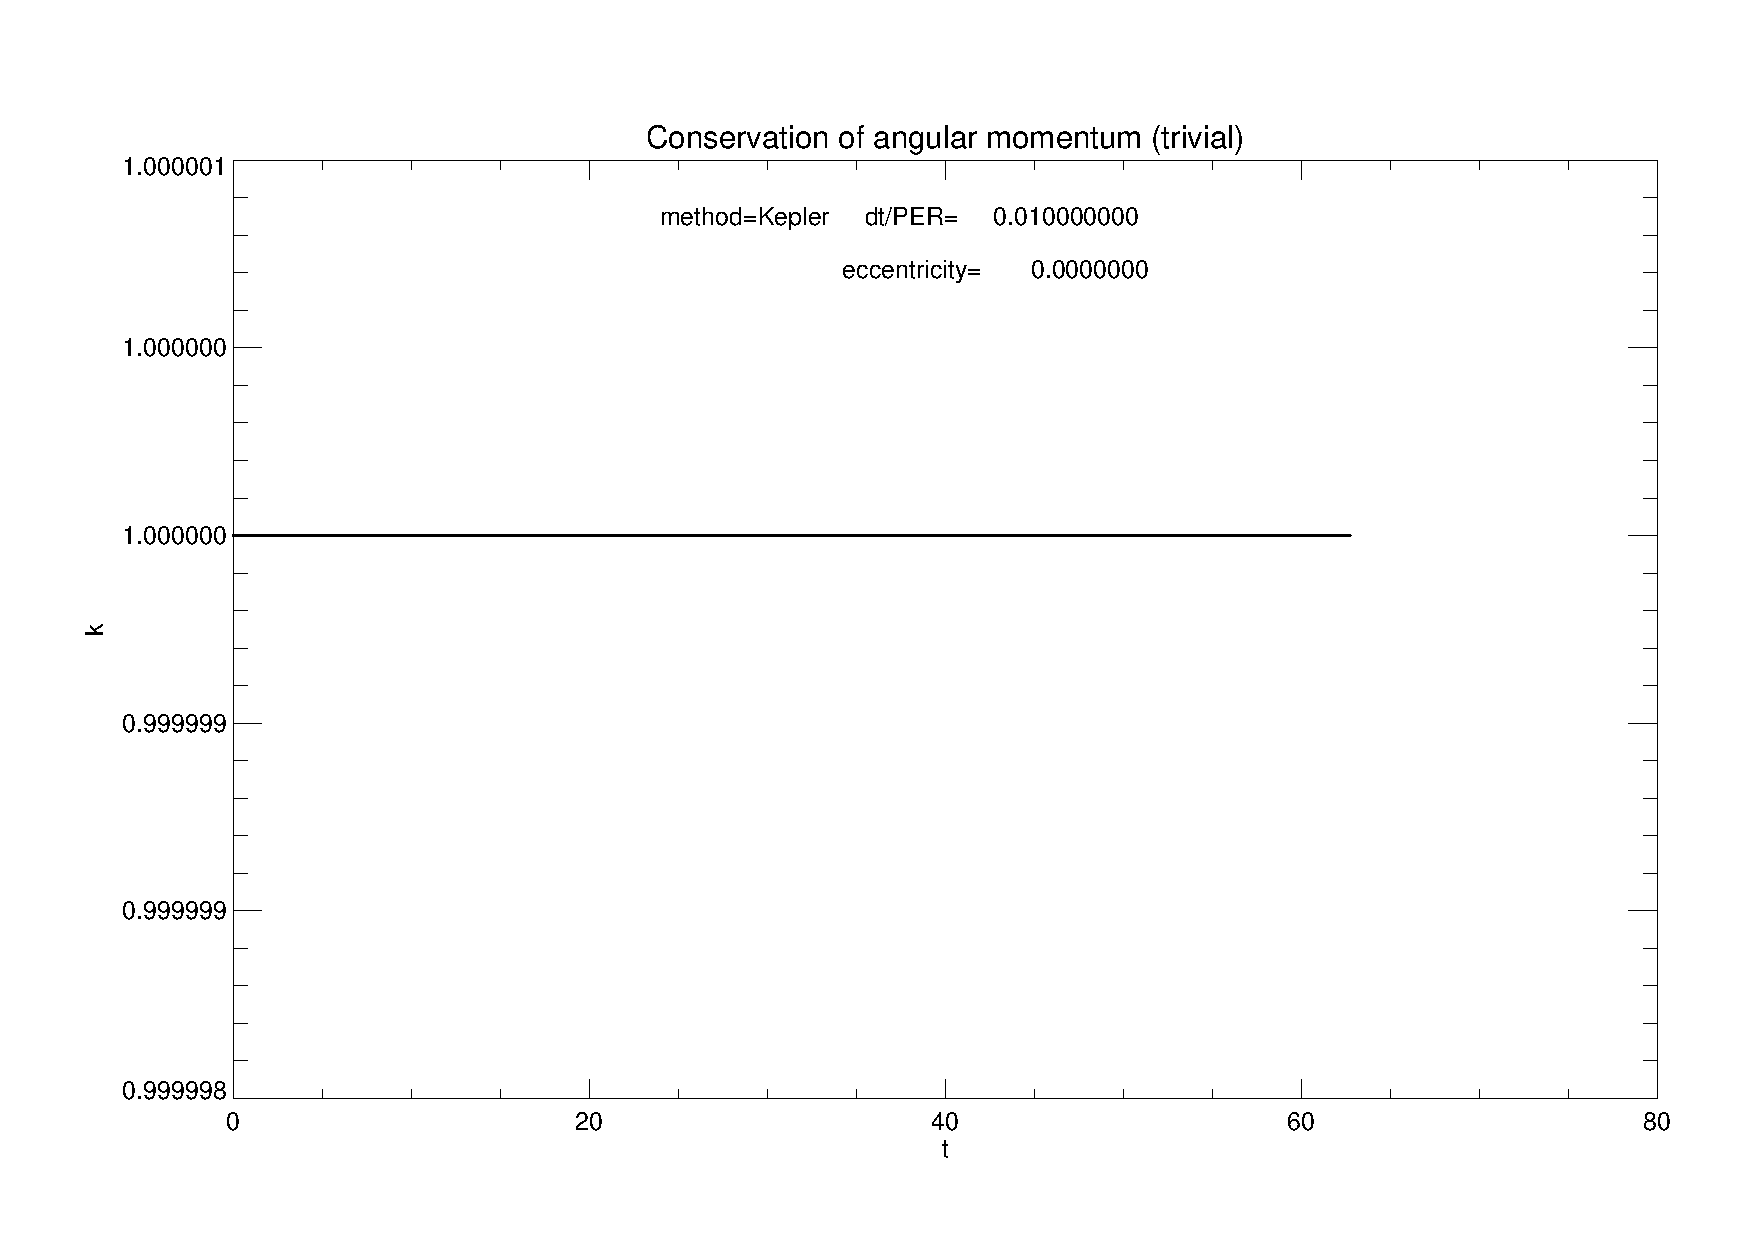
\includegraphics[page=1,angle=0,width=0.7\paperwidth]{numorb_angmom.pdf}%}
\end{figure}

\begin{figure}[H]%\centerline{
\vspace*{-2cm}
\includegraphics[page=2,angle=0,width=0.7\paperwidth]{numorb_angmom.pdf}%}
\caption{Analyyttinen rata ja 1. kertaluvun Taylorin menetelmä $dt=0.01P$}
\end{figure}

\newpage
\begin{figure}[H]%\centerline{
%\vspace*{-2.5cm}
\includegraphics[page=3,angle=0,width=0.7\paperwidth]{numorb_angmom.pdf}%}
\end{figure}

\begin{figure}[H]%\centerline{
\vspace*{-2cm}
\includegraphics[page=4,angle=0,width=0.7\paperwidth]{numorb_angmom.pdf}%}
\caption{2. kertaluvun Taylorin menetelmä ja Runge-Kutta, $dt=0.01P$}
\end{figure}

\newpage
\section[Tehtävä 2b]{Kahden kappaleen liike $1/r^3$ -voimakentässä}

\newpage
\section{Käytetyt ohjelmat}

\subsection[Koodi1]{Ohjelman mars.pro sisältö}\label{Koodi1}
\begin{scriptsize}
\begin{verbatim}
;----------------------------------------------------------------------;
; TAIVAANMEKANIIKAN KOTITEHTÄVÄT (vm 2012)
;----------------------------------------------------------------------;
; Osa 1) Marsin rata taivaalla vuosina 2000-2020
;------------------------------------------------------------------------;
; Use the subroutine PsPlot to save results in a postscript plot 
;------------------------------------------------------------------------;
pro PsPlot,routine,filename
	thisdir=getenv('PWD')+'/'
	psopen,/color,dir=thisdir,filename
	call_procedure,routine
	psclose		
end

;------------------------------------------------------------------------;
;  MAIN PROGRAM starts here
;------------------------------------------------------------------------;
pro mars

;------------------------------------------------------------------------;
; TIME between 2000-2020 (21 years)
;------------------------------------------------------------------------;
; In years (0.01yr interval)
timet=dindgen(2100)/100.d0
; In days
tday=timet*365.25d0
; In centuries (functions as Julian centuries, technically should
; substract t=J-2451545.0 though)
tcen=tday/36525.d0

;------------------------------------------------------------------------;
; Elements in eplictic and equatorial systems
;------------------------------------------------------------------------;
;Declination
deltat=timet
;Rectascension
alphat=timet

;Latitude
lattab=timet
;Longitude
lontab=timet

;------------------------------------------------------------------------;
; Loop for solving the orbit starts here
;------------------------------------------------------------------------;
;NOTE: use 'long' type for index i so that the loop won't end
;prematurely

for i=0l,n_elements(timet)-1 do begin

;Time in julian centuries
T=tcen(i)

;------------------------------------------------------------------------;
; Orbital elements of Mars (from Karttunen: Johdatus taivaanmekaniikkaan)
; (time-dependent)
;------------------------------------------------------------------------;
; Semimajor axis (in AU)
a=1.52366231d0-0.0000722d0*T
; Eccentricity
eks=0.09341233d0+0.00011902d0*T
; Inclination (in degrees)
ink=1.85061d0-25.47d0/3600.d0*T
; Longitude of ascending node (in degrees)
ome=49.57854d0-1020.19d0/3600.d0*T
; Longitude of perihelion (in degrees)
wp=336.04084d0+1560.78d0/3600.d0*T
; Longitude (in degrees)
L=355.45332d0+0.52403304d0*tday(i)

; Argument of pericenter
w=wp-ome
; Mean anomaly
M=L-wp

; Time of pericenter (not really needed here since M is given directly,
; but the program input wants it)
tau=0.d0
; All the elements combined
elem_mars=[a,eks,ink,ome,w,tau]

; Corrected mean anomaly (use modulo to loop every 360deg)
M_mars=(M mod 360.d0)/360.d0*2.d0*!dpi

;------------------------------------------------------------------------;
; Orbital elements of Earth (from Karttunen: Johdatus taivaanmekaniikkaan)
;------------------------------------------------------------------------;
; Semimajor axis
a_m=1.00000011d0-0.00000005*T
; Eccentricity
eks_m=0.01671022d0-0.00003804*T
; Inclination
ink_m=0.00005d0-46.94/3600.*T
; Longitude of ascending node (in degrees)
ome_m=-11.26064d0-18228.25/3600.*T
; Longitude of perihelion (in degrees)
wp_m=102.94719d0+1198.28/3600*T
; Longitude (in degrees)
L_m=100.46435d0+0.98560910*tday(i)

; Argument of pericenter
w_m=wp_m-ome_m
; Mean anomaly
M_m=L_m-wp_m

; Elements combined (can use same tau as Mars)
elem_m=[a_m,eks_m,ink_m,ome_m,w_m,tau]

; Corrected mean anomaly (again use modulo)
M_maa=(M_m mod 360.d0)/360.d0*2.d0*!dpi

;--------------------------------------------------------------------------;
; Use the subprogram 'elem_to_rv.pro' to get the radius vector
;--------------------------------------------------------------------------;
; For Mars
time=0.d0
elem_to_rv,elem_mars,time,rad,vel,M0=M_mars
rad_mars=rad

; For Earth
elem_to_rv,elem_m,time,rad_m,vel_m,M0=M_maa
rad_maa=rad_m

;--------------------------------------------------------------------------;
; Get place coordinates in ecliptic system
;--------------------------------------------------------------------------;
; (x,y,z) from substracting (x_mars-x_maa,y_mars-y_maa,z_mars-z_maa)
x=rad_mars(0)-rad_maa(0)
y=rad_mars(1)-rad_maa(1)
z=rad_mars(2)-rad_maa(2)

; Change from (x,y,z) to (r,lat,long)
r=sqrt(x^2+y^2+z^2)
lattab(i)=asin(z/r)*!radeg
lontab(i)=atan(y,x)*!radeg

;---------------------------------------------------------------------------;
; Rotate ~23deg with respect to x axis to get coord. in equator system
;---------------------------------------------------------------------------;
; Angle of Earth's rotational axis (in radians)
ekli=23.43928d0;/!radeg
; Slightly faster to define cos(ekli) and sin(ekli) beforehand
sine=sin(ekli/!radeg)
cose=cos(ekli/!radeg)

; (x',y',z') solved from rotational matrix
; actually 'ekli' should be negative, but the same result is achieved
; by setting sin(ekli) -> -sin(ekli) and cos(ekli) -> cos(ekli) in the
; rotation matrix
xe=x
ye=y*cose-z*sine
ze=y*sine+z*cose

; Change from (x',y',z') to (r,delta,alpha)
re=sqrt(xe^2+ye^2+ze^2)
delta=asin(ze/re)*!radeg
alpha=atan(ye,xe)*!radeg

; Make sure that the rectascension is not negative
if (alpha le 0) then alpha=alpha+360.d0

; Add current values to the tables defined in the beginning of program
deltat(i)=delta
alphat(i)=alpha

; END THE LOOP finally
endfor

;--------------------------------------------------------------------;
; Draw the orbit (ecliptic)
;--------------------------------------------------------------------;
nwin
plot,lontab,lattab,xtitle='Longitudi pitkin ekliptikaa',$
title='Marsin rata 2000-2020',ytitle='Latitudi',psym=3

;--------------------------------------------------------------------;
; Check results by using 'planet_coords' procedure in ASTRO-library
;--------------------------------------------------------------------;
; Use julian date
juldate,[2000.,1.,1],jd0 ;gives reduced JD-2400000.0
jd0=jd0+2400000.d0       ;get JD for our starting time
jd=jd0+tday              ;transform used timetable into JD

; From ASTRO-library (two options)
planet_coords,jd,/jd,ra_astro,dec_astro,planet='mars'
;JPL ephemerids did not work?
planet_coords,jd,/jd,ra_jpl,dec_jpl,planet='mars',/jpl

;--------------------------------------------------------------------;
; Declination
;--------------------------------------------------------------------;
nwin
;!p.multi=[0,2,2]
;!p.charsize=0.7

plot,timet+2000,deltat,xr=[0,20]+2000,$
ytitle='Marsin deklinaatio',xtitle='Vuosi',psym=3

;Plot only one in every 20 points
index=lindgen(n_elements(timet)/20)*20

oplot,2000+timet(index),dec_astro(index),psym=6,syms=0.5
oplot,2000+timet(index),dec_astro(index),psym=1,syms=0.5

;--------------------------------------------------------------------;
; Rectascension
;--------------------------------------------------------------------;
nwin
plot,2000+timet,alphat,xr=[0,20]+2000,$
     xtitle='Vuosi',ytitle='Marsin rektaskensio',psym=3
  
oplot,2000+timet(index),ra_astro(index),psym=6,syms=0.5
oplot,2000+timet(index),ra_astro(index),psym=1,syms=0.5

;--------------------------------------------------------------------;
; Errors (compare to JPL)
;--------------------------------------------------------------------;
; For declination
nwin
plot,timet+2000,(deltat-dec_jpl)*60.,xr=[0,20]+2000,$
       xtitle='Vuosi',ytitle='Deklinaation virhe (arcmin)',psym=3
; For rectascension (neglect full round difference)
d_alpha=atan(tan((alphat-ra_jpl)/!radeg))*!radeg
nwin
plot,2000+timet,d_alpha*60,xr=[0,20]+2000,$
       xtitle='Vuosi',ytitle='Rektaskension virhe (arcmin)',psym=3
end

;--------------------------------------------------------------------;
; Save the results to a PostScript file using PsPlot
;--------------------------------------------------------------------;
pro Plot_everything
PsPlot, 'mars', 'mars.ps'
end

\end{verbatim}
\end{scriptsize}

\end{document}